\chapter{Background}		
\label{chapter2}


\section{Heading}

\begin{paragraph}
The chapter headings should be 14 points and any other titles should be in 12 points.  The text in the chapter body should be computer printed in 12 points Times New Roman font.
\end{paragraph}

\subsection{Sub-heading 1}

\begin{subparagraph}
Typing should be with a spacing of 1.5 between lines, including the List of References and Appendices.
\end{subparagraph}






\subsubsection{Sub-heading 2}

\begin{subsubparagraph}
Subheading 2 provides an example of items presented in an enumerated list.
\end{subsubparagraph}

\begin{enumerate}[itemindent=\subsubparitemindent]
\item Enumerate One
\item Enumerate Two
\item Enumerate Three
\end{enumerate}


\section{Equation} 

\begin{paragraph}
As an illustration of \LaTeX's mathematics formatting,
\autoref{ch2:eq:renyi} is the definition of {\em R\'enyi entropy} and \autoref{ch2:eq:total-loss} is the total loss function:
\end{paragraph}

%%%%%%%%%%%%%%%%%%%%%%%%% EQUATION  %%%%%%%%%%%%%%%%%%%%%%%%% 
\begin{equation}
\label{ch2:eq:renyi}
H_{\alpha}(X) =
\frac{1}{1-\alpha}
\log \left(\sum_{x \in {\cal X}}P[X=x]^{\alpha} \right) .
\end{equation}

%%%%%%%%%%%%%%%%%%%%%%%%%  EQUATION %%%%%%%%%%%%%%%%%%%%%%%%% 
\begin{equation} 
\label{ch2:eq:total-loss}
\begin{aligned}
\mathcal{L}_{\textrm{total}} = \frac{1}{N}\sum_{i=1}^{N}\{w_i\mathcal{L}_i\}. 
\end{aligned}
\end{equation}


\section{Algorithm}

\begin{paragraph}
This is an example of \autoref{ch2:algo:my-algo}.
\end{paragraph}

\begin{algorithm}[h]
\caption{An algorithm with caption.}
\label{ch2:algo:my-algo}
\normalsize\singlespacing
\begin{algorithmic}[1] % [1] print number all lines 
    \Require $n \geq 0$
    \Ensure $y = x^n$
    \State $y \gets 1$
    \State $X \gets x$
    \State $N \gets n$
    \While{$N \neq 0$}
    \If{$N$ is even}
        \State $X \gets X \times X$
        \State $N \gets \frac{N}{2}$  \Comment{This is a comment}
    \ElsIf{$N$ is odd}
        \State $y \gets y \times X$
        \State $N \gets N - 1$
    \EndIf
    \EndWhile
\end{algorithmic}
\end{algorithm}



\section{The table numbers}

\begin{paragraph}
The table numbers shall represent the chapter numbers. For example, the first table in the \autoref{chapter2} shall be ``\autoref{ch2:table:results} ...................'', etc. The number and title of a table (Table caption) should be placed ABOVE the table and aligned left. The word ``\autoref{ch2:table:results}'' is \textbf{bold} font except its caption. 
\end{paragraph}

%%%%%%%%%%%%%%%%%%%%%%%%% TABLE BEGIN %%%%%%%%%%%%%%%%%%%%%%%%% 
%%%%% Create LaTeX table from https://www.tablesgenerator.com/
\begin{table}[ht]
\caption{Classification performance.}
\label{ch2:table:results}
\centering
\normalsize\singlespacingplus
    \begin{tabular}{@{}ccc@{}}
    \toprule
    \multirow{2}{*}{\textbf{Comparison Model}} & \multicolumn{2}{c}{\textbf{Subject-independent}}       \\ \cmidrule(l){2-3} 
                                               & \textbf{Accuracy $\pm$ SD}          & \textbf{F1-score $\pm$ SD}         \\ \midrule
    FBCSP-SVM                                  & $64.96 \pm 12.70$          & $65.25 \pm 15.14$         \\
    Deep Convnet                               & $68.33 \pm 15.33$          & $70.20 \pm 15.18$         \\
    EEGNet-8,2                                 & $68.84 \pm 13.87$          & $70.39 \pm 14.30$         \\
    Spectral-Spatial CNN                       & $68.27 \pm 13.56$          & $65.86 \pm 17.37$         \\
    MIN2Net                                    & $\mathbf{72.03 \pm 14.04^*}$ & $\mathbf{72.62 \pm 14.14^*}$ \\ \bottomrule
    \end{tabular}%
\end{table}
%%%%%%%%%%%%%%%%%%%%%%%%% TABLE END %%%%%%%%%%%%%%%%%%%%%%%%%  





\section{The figure numbers}

\begin{paragraph}
The figure numbers shall represent the chapter numbers. For example, the first figure in \autoref{chapter2} shall be ``\autoref{ch2:fig:model}'', etc. the number and title of a figure (Figure caption) should be placed BELOW the figure. For the figure caption which contains only 1 line, it should align CENTER throughout the thesis. For the figure caption which contains more than 1 line, it should align left throughout the thesis. The figure format should be pdf, png, jpg or \lstinline[language=C]!\chemfig! as \autoref{ch2:fig:mychemfig}
\end{paragraph}


%%%%%%%%%%%%%%%%%%%%%%%%% FIGURE BEGIN %%%%%%%%%%%%%%%%%%%%%%%%% 
\begin{figure}[ht]
\centering
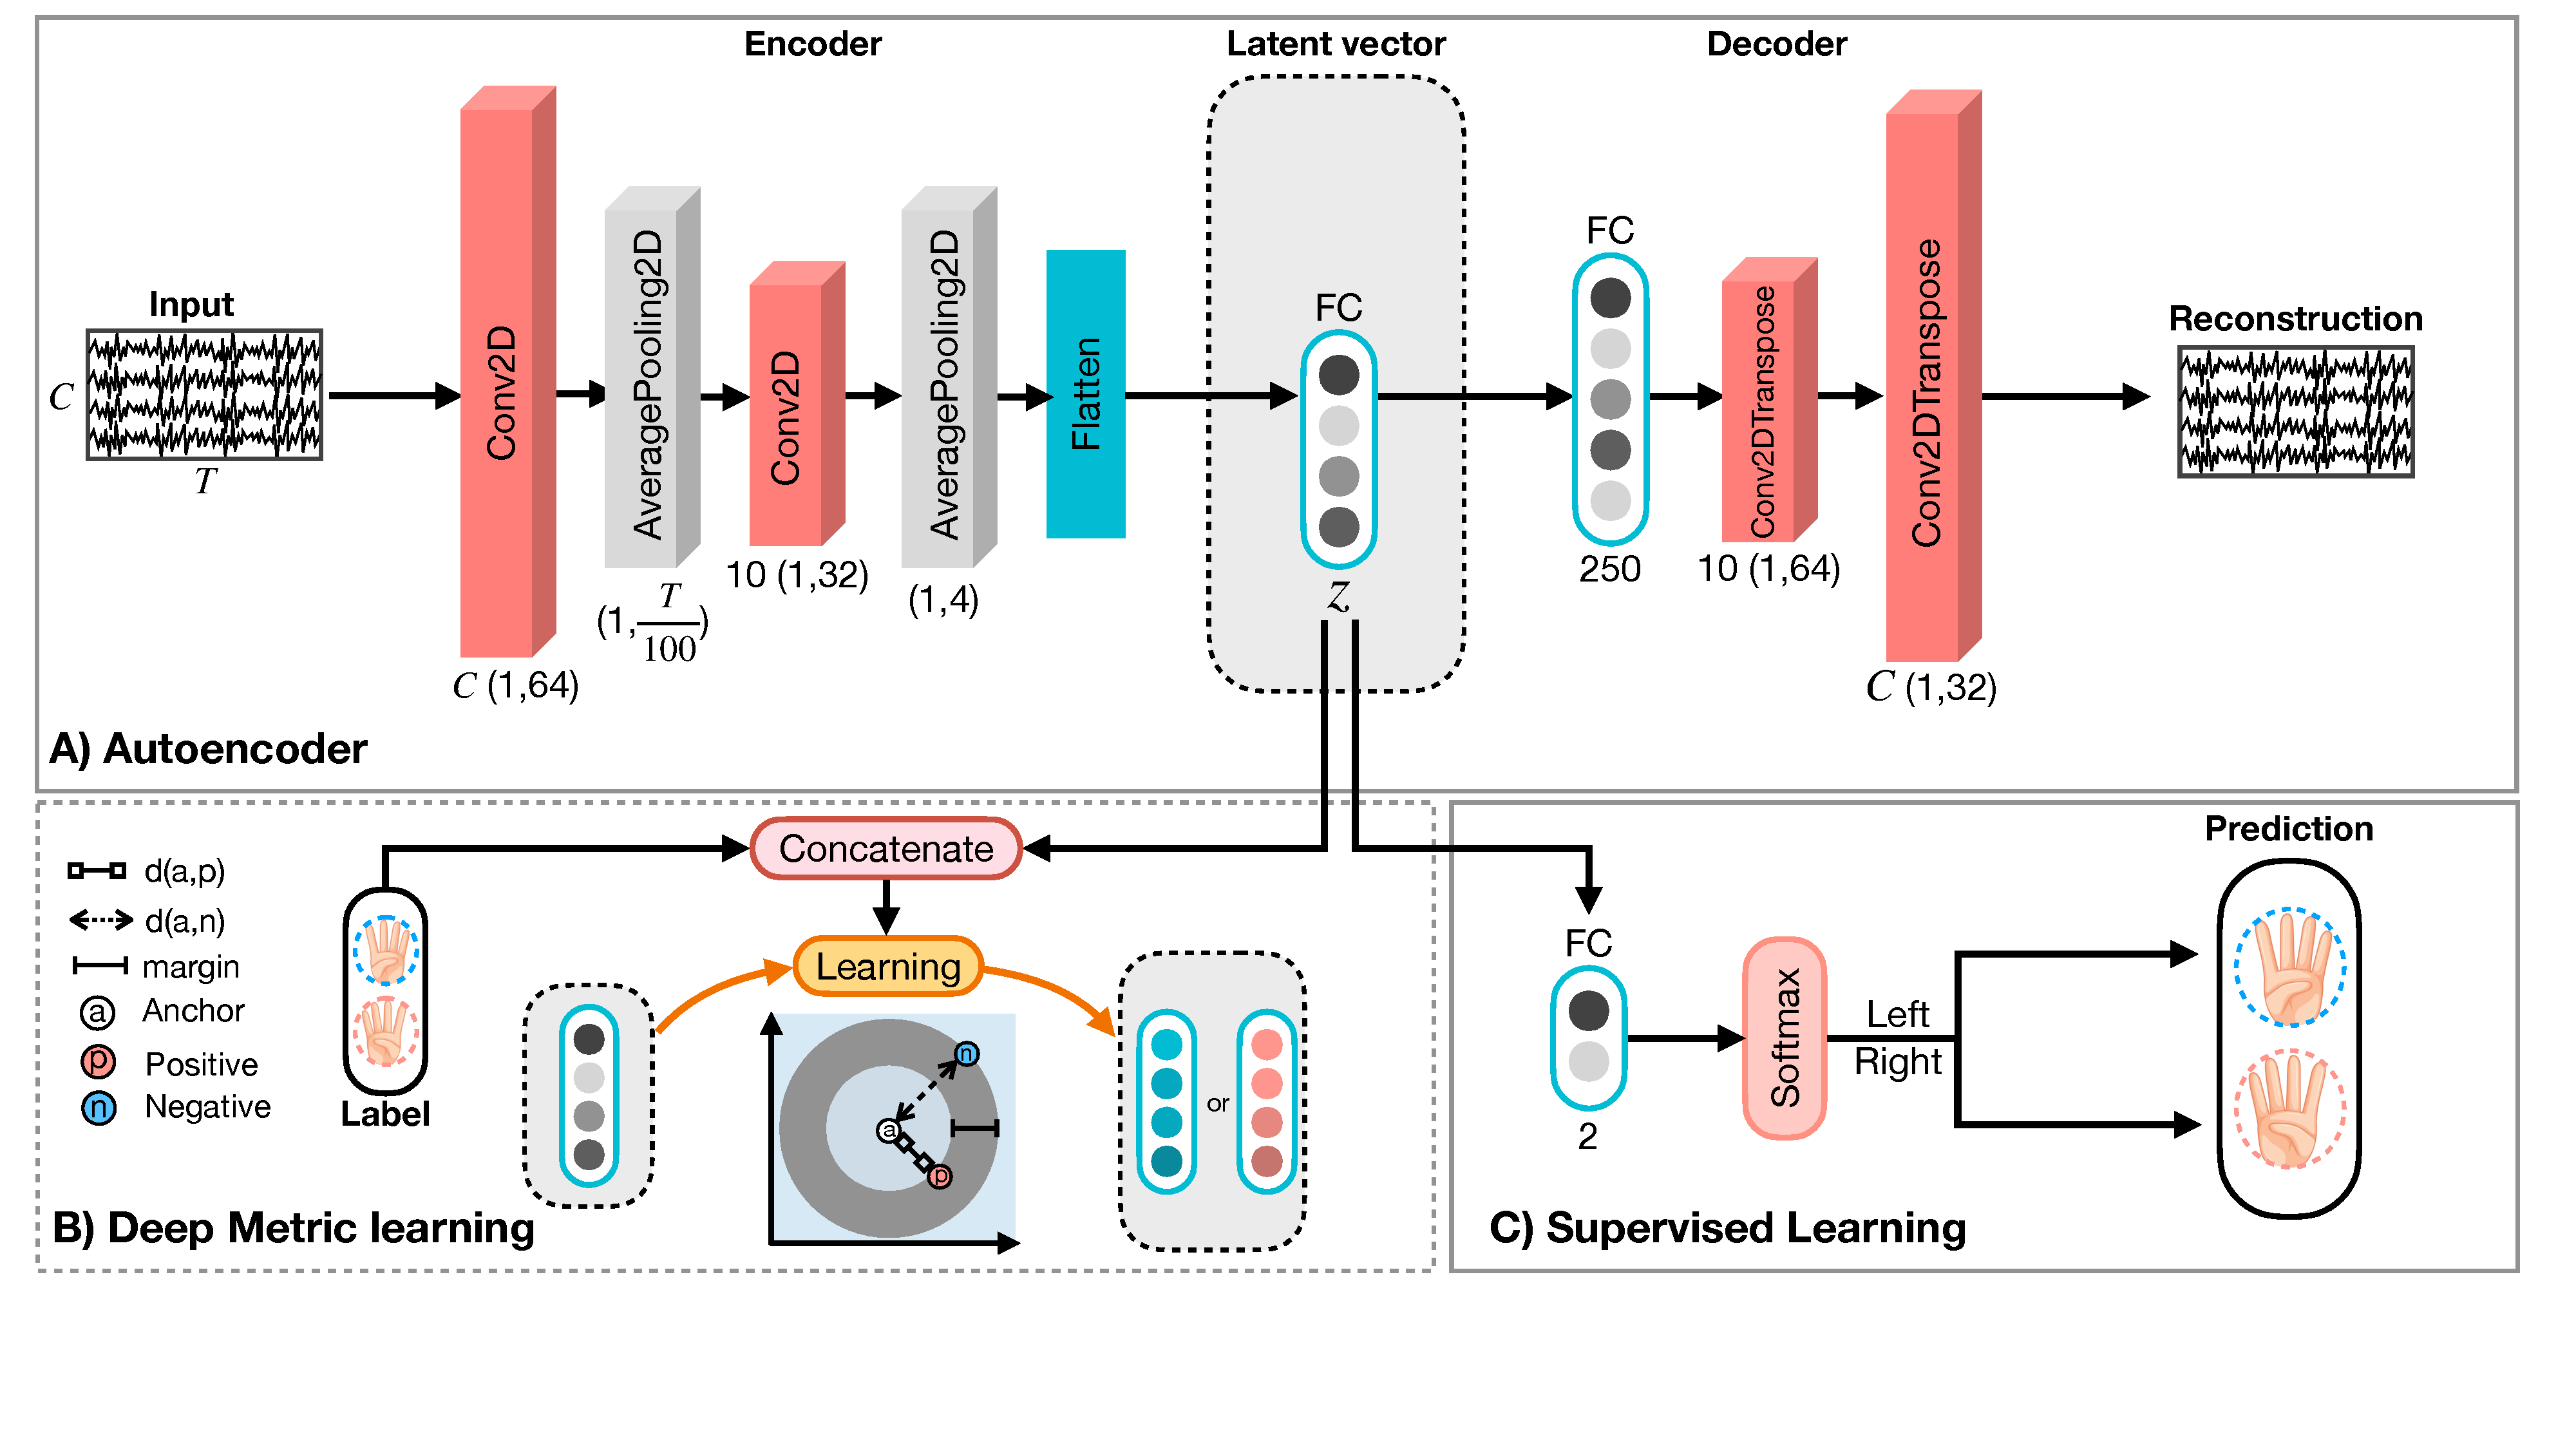
\includegraphics[width=1\columnwidth]{figures/ch2/model.pdf}
\longcaption[The MIN2Net model architecture.]{An overview of the MIN2Net model architecture. The figure illustrates the sequence of processing blocks, including the temporal convolutional layers, feature extraction modules, and classification layers. Each component is annotated to reflect its role in the end-to-end EEG signal processing pipeline.}
\label{ch2:fig:model}
\end{figure}
%%%%%%%%%%%%%%%%%%%%%%%%% FIGURE END %%%%%%%%%%%%%%%%%%%%%%%%% 


%%%%%%%%%%%%%%%%%%%%%%%%% FIGURE BEGIN %%%%%%%%%%%%%%%%%%%%%%%%% 
\begin{figure}[ht]
    \centering
    % From the documentation
    % https://ctan.mirror.garr.it/mirrors/ctan/macros/generic/chemfig/chemfig-en.pdf
    \chemnameinit{\chemfig{R-C(-[:-30]OH)=[:30]O}}
    \schemestart
    \chemname{\chemfig{R’OH}}{Alcohol}
    \+
    \chemname{\chemfig{R-C(-[:-30]OH)=[:30]O}}{Carboxylic acid}
    \arrow(.mid east--.mid west)
    \chemname{\chemfig{R-C(-[:-30]OR’)=[:30]O}}{Ester}
    \+
    \chemname{\chemfig{H_2O}}{Water}
    \schemestop
    \chemnameinit{}
    \caption{The caption on this figure, the second and other lines need to be aligned with the first letter of the first line.}
    \label{ch2:fig:mychemfig}
\end{figure}


\section{Citations}
\begin{paragraph}
This is an example of how to cite previous work, such as \cite{min2net}, or multiple sources like \cite{hu79, somework2020, tonio_paper}. Ensure that the corresponding BibTeX entries are added to the \texttt{bibliography.bib} file before citing.

Below is an example BibTeX entry:

\begin{verbatim}
@ARTICLE{min2net,
  author  = {Autthasan, Phairot and Chaisaen, Rattanaphon and 
            Sudhawiyangkul, Thapanun and Rangpong, Phurin and 
            Kiatthaveephong, Suktipol and Dilokthanakul, Nat 
            and Bhakdisongkhram, Gun and Phan, Huy and Guan, 
            Cuntai and Wilaiprasitporn, Theerawit},
  journal = {IEEE Transactions on Biomedical Engineering}, 
  title   = {MIN2Net: End-to-End Multi-Task Learning for Subject-
            Independent Motor Imagery EEG Classification}, 
  year    = {2022},
  volume  = {69},
  number  = {6},
  pages   = {2105-2118}
}
\end{verbatim}

\end{paragraph}

